% !TEX spellcheck = en_US

\documentclass[conference]{IEEEtran}
\usepackage{cite}
\usepackage{amsmath,amssymb,amsfonts}
\usepackage{algorithmic}
\usepackage{graphicx}
\usepackage{textcomp}
\usepackage{xcolor}
% add hyperlinks, delete all .aux files if adding hyperref after previous build
\usepackage{hyperref}
% support for unicode charcters like "é" and "ñ"
\usepackage[T1]{fontenc}
% Provides generic commands \degree, \celsius, \perthousand, \micro and \ohm
\usepackage{gensymb}
% splits a section into multiple columns
\usepackage{multicol}
\def\BibTeX{{\rm B\kern-.05em{\sc i\kern-.025em b}\kern-.08em
    T\kern-.1667em\lower.7ex\hbox{E}\kern-.125emX}}
\begin{document}

\title{Tracker Terrain Loss Part Two}

\author{\IEEEauthorblockN{Mark A. Mikofski and Rounak Kharait}
	\IEEEauthorblockA{DNV, Oakland, CA, 9612, USA }}

\maketitle

\begin{abstract}
Write an abstract
\end{abstract}

\begin{IEEEkeywords}
TMY, SURFRAD, irradiance, performance, prediction
\end{IEEEkeywords}

\section{Introduction}
Write an introduction

\section{Methods}
Write about the methods

\section{Results}
Write about the results

\begin{figure}[htbp]
\centerline{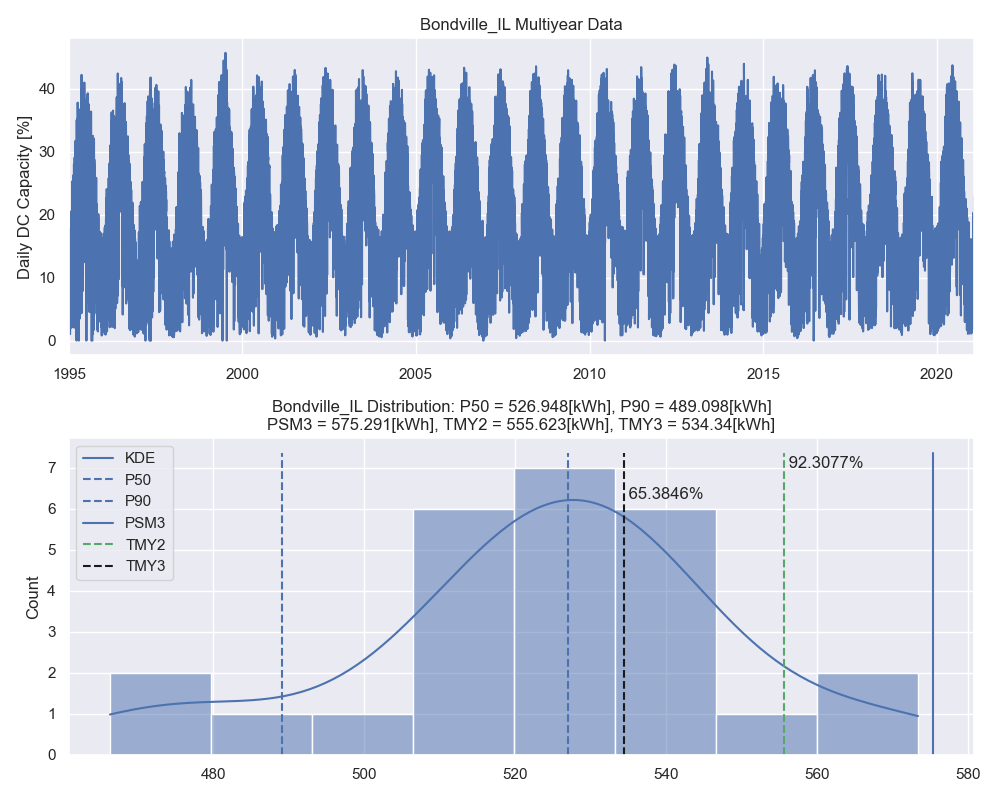
\includegraphics[width=9cm]{Bondville_IL.png}}
\caption{Daily capacity factor relative to DC nameplate for Bondville, IL, SURFRAD site (top) and distribution of annual DC energy per module (bottom).}
\label{fig:Bondville-IL}
\end{figure}

\begin{figure}[htbp]
\centerline{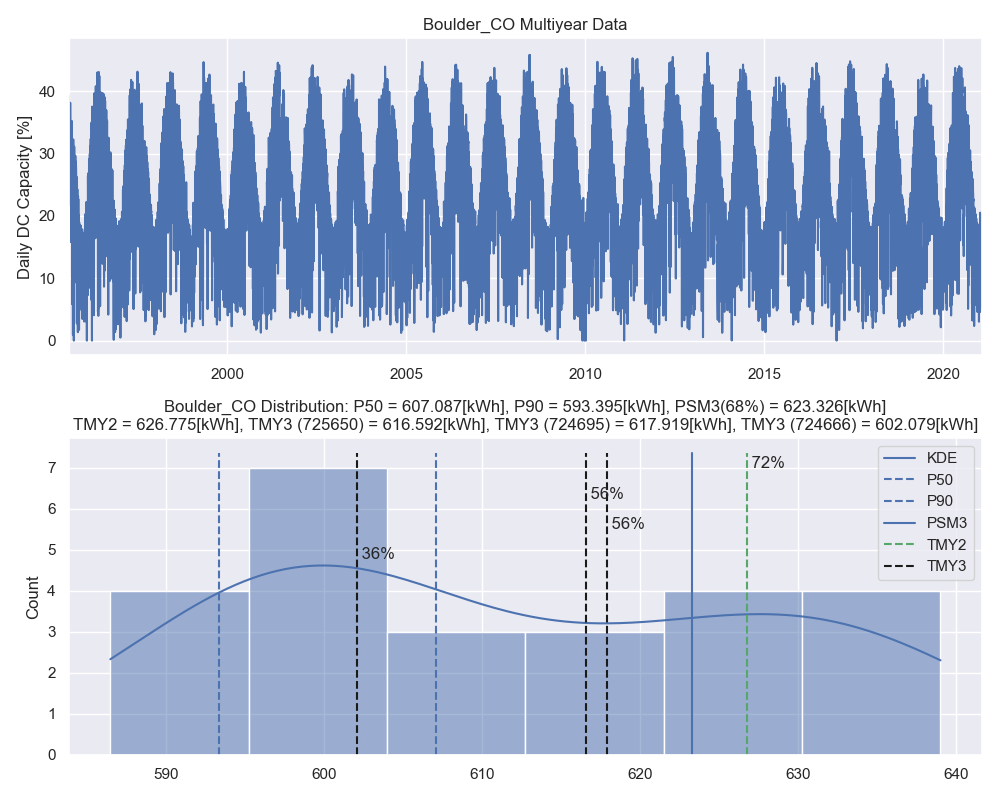
\includegraphics[width=9cm]{Boulder_CO.png}}
\caption{Daily capacity factor relative to DC nameplate for Boulder, CO, SURFRAD site (top) and distribution of annual DC energy per module (bottom).}
\label{fig:Boulder-CO}
\end{figure}

\begin{figure}[htbp]
\centerline{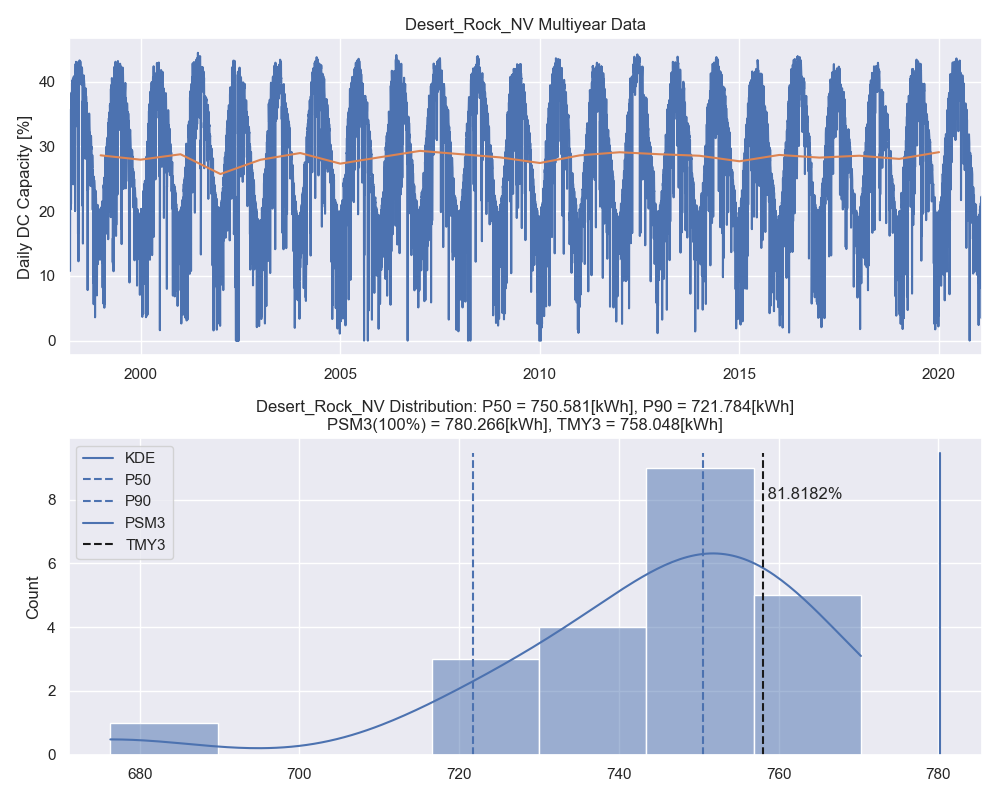
\includegraphics[width=9cm]{Desert_Rock_NV}}
\caption{Daily capacity factor relative to DC nameplate for Desert Rock, NV, SURFRAD site (top) and distribution of annual DC energy per module (bottom).}
\label{fig:Desert-Rock-NV}
\end{figure}

\begin{figure}[htbp]
\centerline{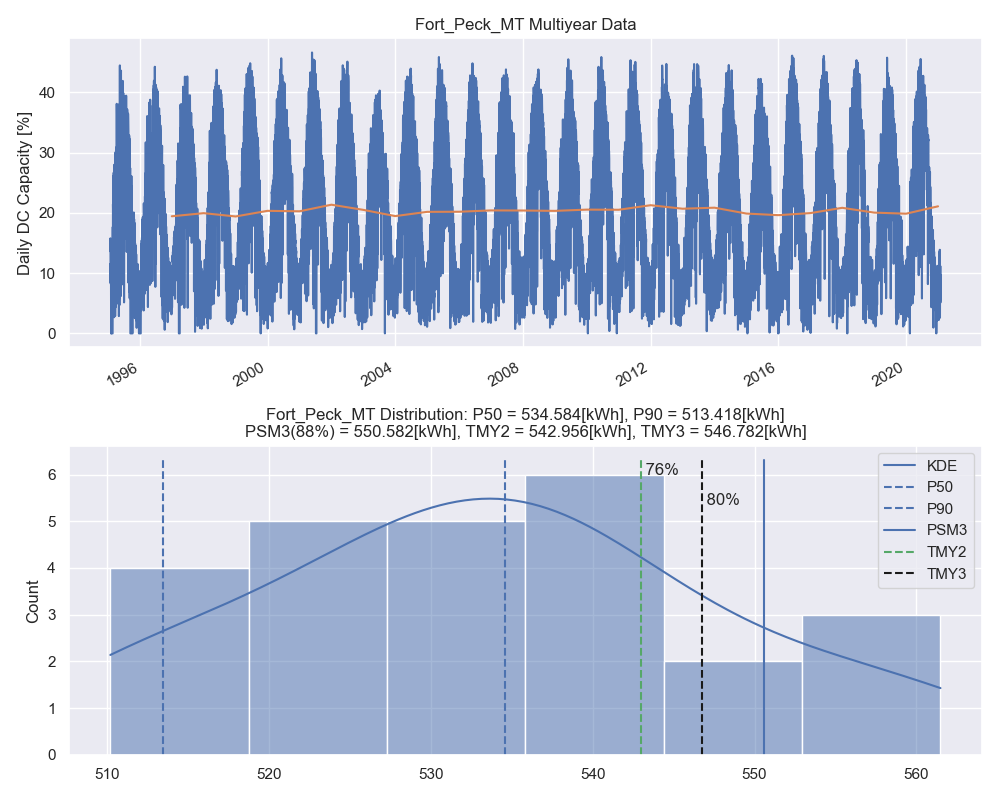
\includegraphics[width=9cm]{Fort_Peck_MT.png}}
\caption{Daily capacity factor relative to DC nameplate for Fort Peck, MT, SURFRAD site (top) and distribution of annual DC energy per module (bottom).}
\label{fig:Fort-Peck-MT}
\end{figure}

\begin{figure}[htbp]
\centerline{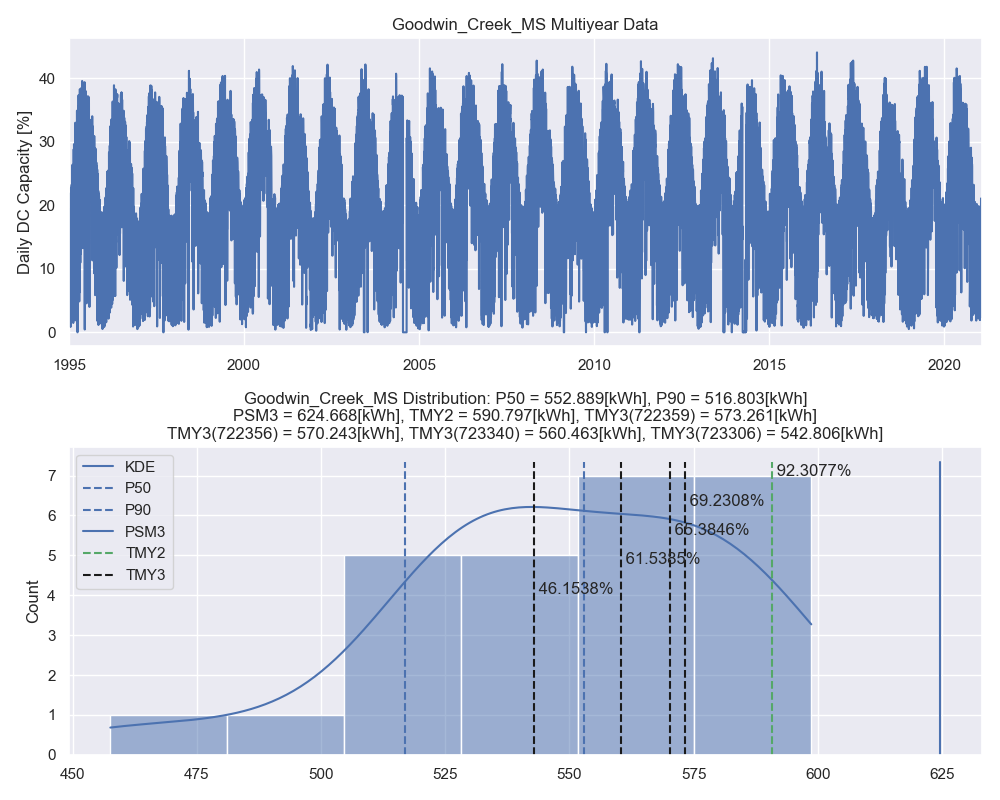
\includegraphics[width=9cm]{Goodwin_Creek_MS.png}}
\caption{Daily capacity factor relative to DC nameplate for Goodwin Creek, MS, SURFRAD site (top) and distribution of annual DC energy per module (bottom).}
\label{fig:Goodwin-Creek-MS}
\end{figure}

\begin{figure}[htbp]
\centerline{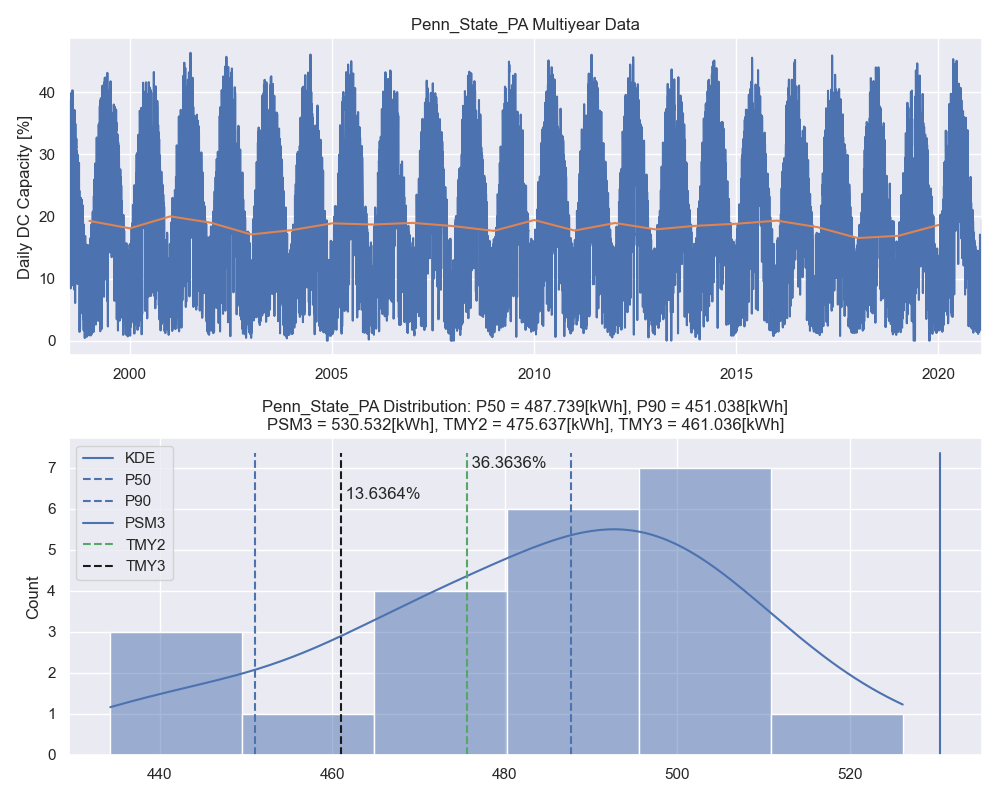
\includegraphics[width=9cm]{Penn_State_PA.png}}
\caption{Daily capacity factor relative to DC nameplate for Penn State, PA, SURFRAD site (top) and distribution of annual DC energy per module (bottom).}
\label{fig:Penn-State-PA}
\end{figure}

\begin{figure}[htbp]
\centerline{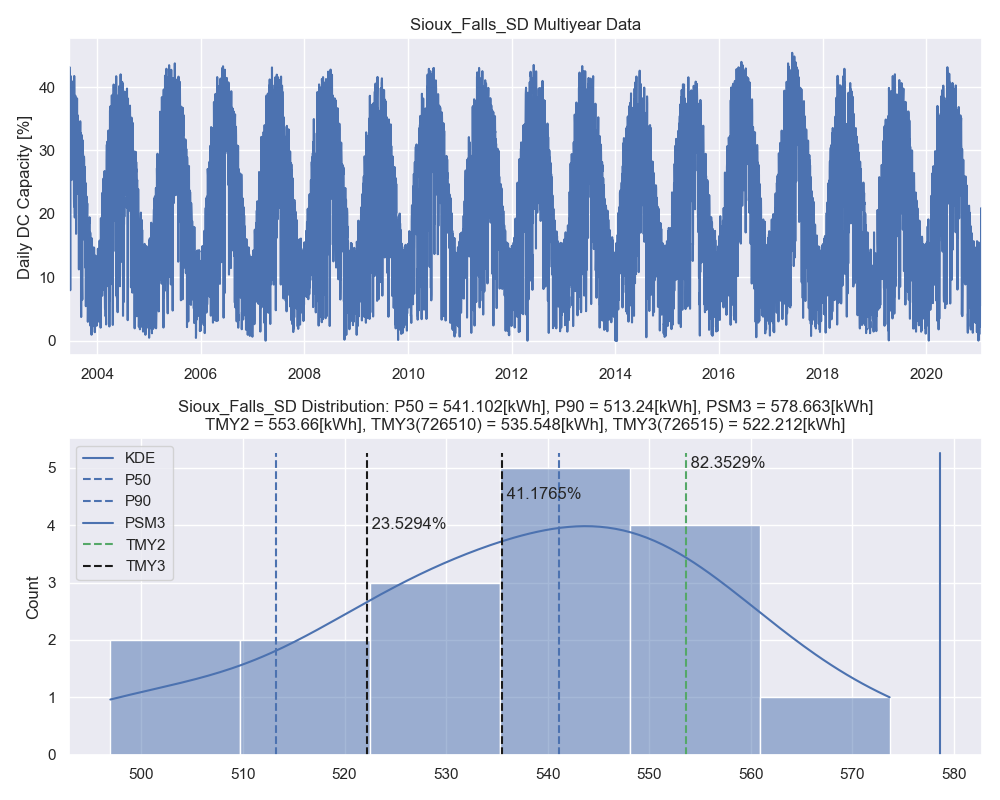
\includegraphics[width=9cm]{Sioux_Falls_SD.png}}
\caption{Daily capacity factor relative to DC nameplate for Sioux Falls, SD, SURFRAD site (top) and distribution of annual DC energy per module (bottom).}
\label{fig:Sioux-Falls-SD}
\end{figure}

\begin{table}[htbp]
\caption{Summary of Predicted SURFRAD Medians Compared with TMY}
\begin{center}
\begin{tabular}{|c|c|c|c|c|}
\hline
\textbf{SURFRAD Station} & \textbf{\textit{P50}}& \textbf{\textit{PSM3}}& \textbf{\textit{TMY2}}& \textbf{\textit{TMY3}} \\
\hline
Bondville, IL    & 20.1\%& 21.9\%& 21.1\%& 20.3\% \\
Boulder, CO      & 23.1\%& 23.7\%& 23.8\%& 23.5\% \\
Desert Rock, NV  & 28.3\%& 29.6\%&       & 28.7\% \\
Fort Peck, MT    & 20.2\%& 21.0\%& 20.7\%& 20.4\% \\
Goodwin Creek, MS& 21.0\%& 23.8\%& 22.5\%& 21.8\% \\
Penn State, PA   & 18.5\%& 20.1\%& 18.1\%& 17.4\% \\
Sioux Falls, SD  & 20.6\%& 22.0\%& 21.1\%& 20.4\% \\
\hline
\end{tabular}
\label{table:surfrad-tmy-summary}
\end{center}
\end{table}

\begin{equation}
E_\text{daily} = \sum_\text{time=1AM}^\text{12AM}{E_\text{hourly}} \label{eq:daily-enregy}
\end{equation}

\begin{equation}
\mathit{CP}_\text{daily} = \frac{E_\text{daily}}{ 24\text{[h]} \text{Nameplate[W]} } \label{eq:daily-capacity-factor}
\end{equation}

\begin{equation}
E_\text{annual }= \sum_\text{day=1}^\text{365}{E_\text{daily}} \label{eq:annual-energy}
\end{equation}

\begin{equation}
\mathit{CP}_\text{annual} = \frac{E_\text{annual}}{ 8760\text{[h]} \text{Nameplate[W]} } \label{eq:annual-capacity-factor}
\end{equation}

\section{Conclusions}
Write the conclusions

\bibliographystyle{IEEEtran}
% argument is your BibTeX string definitions and bibliography database(s)
\bibliography{IEEEabrv,bibliography}

\end{document}
